\documentclass{tudphygp_eng}
\usepackage{tudphymd,mhchem}

\versuch{Diffusion}{DI}
\author{K.~Prokert}
\bearbeitet{M.~Lange,S.~Socher,engl. S.~Saager}{}

\begin{document}
\maketitle

\section{Task}

The diffusion coefficient between \ce{NaCl}- solution and distilled water has to be determined by schlieren method after \textsc{Wiener}.

\section{Fundamentals}

\subsection{Diffusion Equation}

If two different but solvable liquids will be superposed above each other, the former sharp interface will blur more and more with time. This mutual mixing process is caused by the motion of the molecules due their thermal energy and is called diffusion.    
\piccaption{ Mass transport during diffusion \label{mtransport}}
 \parpic[r]{
  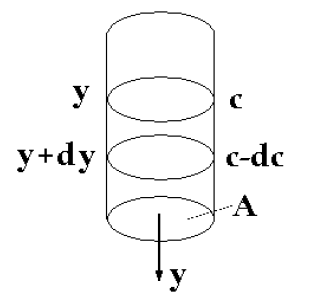
\includegraphics[width=4.5cm]{GP2-DI-abb1.png} 
 }
Let's assume a cylinder with the cross section area $A$ (Fig. \ref{mtransport}) and with symmetric axis parallel to $y$-direction. Let's assume further the concentration at the level $y$ is $c$ and at the nearby level $y+dy$ the concentration is $c-dc$. Then there exist a concentration gradient between these two levels and the amount of substance $dN$ (in mole) which runs through the area $A$ per time unit $dt$ can be expressed by the 1. \textsc{Fick}'s law (published in 1855): %(Eq.\ref{1ficklaw})

\begin{equation} \label{1ficklaw}
dN= - D \cdot A \dfrac{dc}{dy} dt
\end{equation}
\picskip{0}
The value $D$ will be called diffusivity or diffusion coefficient.

The temporal profile of diffusion will be described by the 2. \textsc{Fick}'s law. Assuming that the interfaces between the two liquids are in close contact at the time $t$ and at the level $y=0$ the concentration $c$ will be a function of time $t$ as well as a function of position $y$. In this case the process will be described by following differential equation:

\begin{equation} \label{diffgl}
\frac{\partial c}{\partial t} = D \cdot \frac{\partial^2 c}{\partial y^2}
\end{equation}

Most of the diffusion processes occurring in reality have to be considered after eq. (\ref{diffgl}). Only special reactions can analysed by the 1. \textsc{Fick}'s law.

\subsection{ Calculation of the Diffusion Coefficient }

If a light ray $L$ passes a media with a sequence of plane-parallel layers of finite thickness and of continuous changing refractive index, then a multiple refraction path will be built up.  
Only in homogeneous media it is allowed to apply the Snell's law, which can be derived from the fundamental law of wave propagation by \textsc{Huygens} principle. In the case of an optical media with continuously changing of refractivity the \textsc{Huygens} principle has to be assumed. 
 
 \piccaption{Applying the \textsc{Huygens} principle
 \label{abb2}}
 \parpic[r]{
  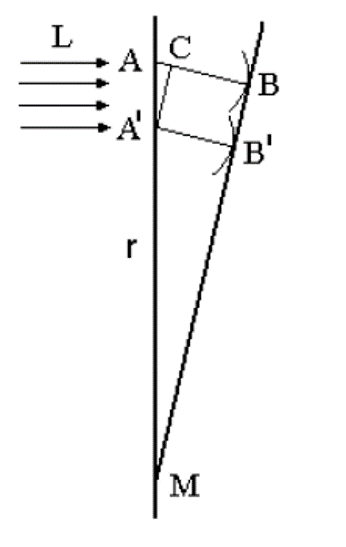
\includegraphics[height=5.0cm]{GP2-DI-abb2_en.png}
 } 
 
Let be $A$ and $A^{'}$ two points (Fig. \ref{abb2}) on the propagating wavefront of the light ray, which enters the media in horizontal direction. They build up agitation centers for two elementary waves moving with different velocities $v$ and $v^{'}$.
After infinitesimal short time $dt$ the wavefront passes the mutual tangent $BB^{'}$. The intersection $M$ of $BB^{'}$ and $AA^{'}$ coincide with the light rays center of curvature.\\
The distance of $A$ to $M$, which is the radius of curvature, can be calculated due to the similarity of the triangles $ABM$ and $ACA^{'}$ . By replacing the distance $AA^{'}$ to $dy$ and by replacing $v$ and $v^{'}$ to $dc$ it follows:

\begin{equation}
\frac{dy}{r} = \frac{dv}{v}.
\end{equation}

With 

\begin{equation}
\left| \frac{dv}{v} \right| = \frac{dn}{n} \quad \text{and} \quad 
 \left| \frac{dy}{r} \right| = \frac{dn}{n}
\end{equation}

it finally results in

\begin{equation} \label{kruemmung}
\frac{1}{r} = \frac{1}{n} \cdot \frac{dn}{dy}   .
\end{equation}

In some cases in a solution the relation between concentration and refraction can be combined to evaluate diffusion profile, because for monochromatic light the refractive index depends on the density number of active molecules.\\





Accordingly in the diffusion zone of two solvable liquids concentration as well as refractive index changes continuously. In this region with a refractivity gradient curved light rays will be observed. \\
Fig. \ref{abb3} shows the sector of a cuvette, in which the area between two parallel plates $P_1$ and $P_2$ contains a solution with decreasing concentration according to the upper (positive) $y$-direction.  

\begin{minipage}{\textwidth}
\vspace{0.05\linewidth}
\ifpdf 
\centerline{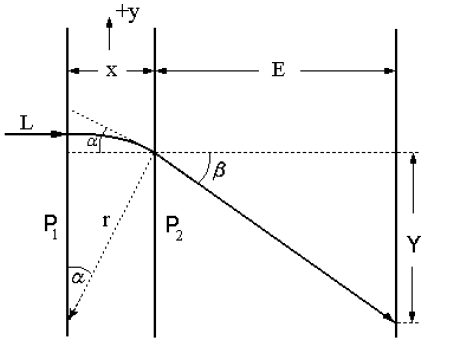
\includegraphics[height=6cm]{GP2-DI-abb3.png}} 
\fi 
\captionof{figure}{ Schematic illustration of a light ray in a medium with  decreasing refractive index in the positive $y$-direction \label{abb3}}
\vspace{0.05\linewidth}
\end{minipage}

A parallel light ray $L$ impinging from the left perpendicular to $P_1$ will be curved into the region of increasing refractivity. The extent of curvature is given by equation (\ref{kruemmung}). $r$ represents the radius of curvature and $n$ the refractive index of the cuvette content at respective position. The incident angle on the interface $P_2$ is no longer perpendicular, hence the light ray will be refracted while the transition to air.

\medskip

Following applies:

\begin{equation} \label{alpha}
\beta = \frac{n}{n_0} \cdot \alpha \quad \text{and} \quad 
\frac{x}{r} \approx \alpha
\end{equation}

thus

\begin{equation}
\beta = \frac{x}{n_0} \cdot \frac{dn}{dy} \approx \frac{Y}{E}
\end{equation}

in which $x$ is the cuvette thickness, $n_0$ the refractive index of air, $E$ the distance between cuvette and screen. $Y$ implies the vertical distance between impingement of refracted light ray and linear prolongation of unrefracted light ray.

\begin{minipage}{\textwidth}
\vspace{0.05\linewidth}
\ifpdf 
\centerline{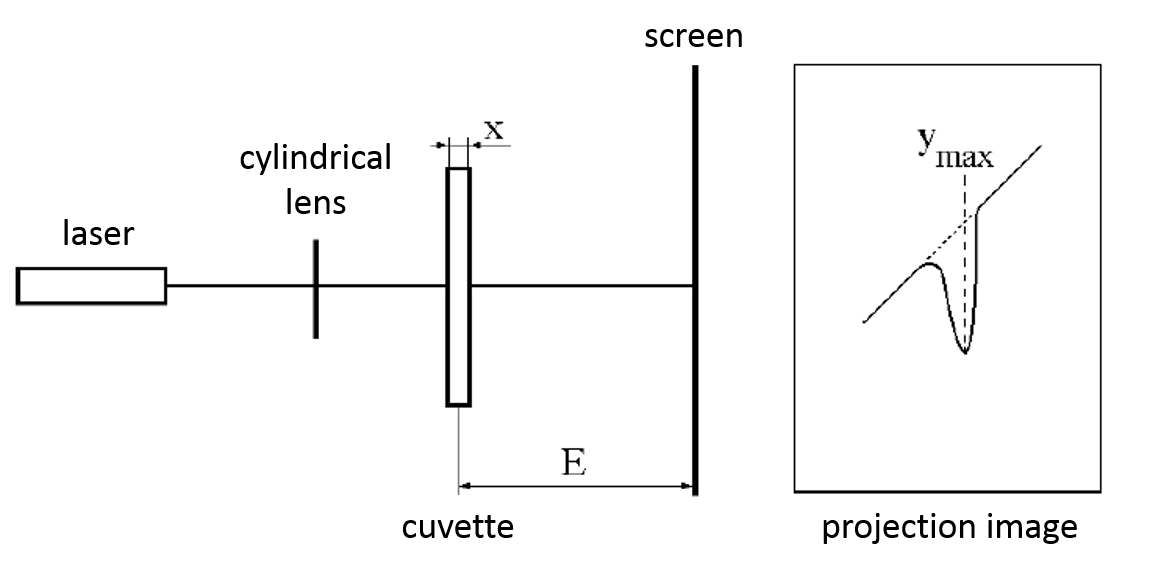
\includegraphics[width=13cm]{GP2-DI-prinzip_en.png}} 
\fi 
\captionof{figure}{Schematic of the experimental setup \label{prinzip}}
\vspace{0.05\linewidth}
\end{minipage}

If the cuvette is filled up half with a solution (refractive index $n_2$) superposed by a other solvable liquid (refractive index $n_1$), both liquid will diffuse into each other with time. It can be assumed, that the resulting refractive index of the mixture is proportional to the concentration $c$. Consequently $c$ in the first and the second \textsc{Fick}'s law can be replaced by the refractive index $n$. 

\medskip

For determination of the diffusion coefficient $D$, you have to integrate equation (\ref{diffgl}). Assuming the interface of both liquids is at the position $y = 0$ for the time $t = 0$, it follows:

\begin{align*}
n=n_1 \quad \text{at} \quad y=+ \infty \\
n=n_2 \quad \text{at} \quad y=- \infty
\end{align*}

and for any other value of $t$:

\begin{equation} \label{brechzahl}
n = \frac{n_1 + n_2}{2} \quad \text{at} \quad y=0
\end{equation}

So we get:

\begin{equation}
n = n_2 + \frac{n_1 - n_2}{2} \cdot \left[ 1 - \frac{2}{\sqrt{\pi}} 
 \int\limits_0^{y/2\sqrt{Dt}} \! \mbox{e}^{{-y^{'}}^2} \, dy^{'} \right] 
\end{equation}

and

\begin{equation}
\frac{dn}{dy} = - \frac{n_1 - n_2}{2 \sqrt{\pi D t}} \cdot \mbox{e}^{- \frac{y^2}{4Dt}}
\end{equation}

At $y=0$ , $\frac{dn}{dy}$ passes a maximum:

\begin{equation}
\left( \frac{dn}{dy} \right)_{y=0} = - \frac{n_1 - n}{2 \sqrt{\pi D t}}
\end{equation}

By inserting of eq. (\ref{brechzahl}) into eq. (\ref{alpha}) it follows a relation for determination of diffusion coefficient:

\begin{equation} \label{diffkoeff}
D = \frac{1}{Y_{max}^2} \cdot \frac{x^2 E^2 (n_1 - n_2)^2}{4 \pi n_0^2 t}
\end{equation}

With this relation it is possible to determine the diffusion coefficient $D$ by plotting the dependence $Y_{max} = f (t)$ in appropriate manner.

\section{Experiment}

In a cuvette K the two liquids will be superposed above each other carefully. A slit S, which has an horizontal inclination of 45�, have to be projected on the screen F. Light rays passing the trough in different levels ($y$-direction) will be deflected variously according to the concentration gradient. The maximal deflection $Y_{max}$ could be measured at the screen (Fig. \ref{prinzip}).
If $Y_{max}$ passes a value of $25 \ldots
30 ~\mathrm{cm}$ data logging can be started.

\medskip

The diffusion cuvette and the reservoir are presented schematically in Fig. \ref{abb4}. 

\begin{minipage}{\textwidth}
\vspace{0.05\linewidth}
\ifpdf 
\centerline{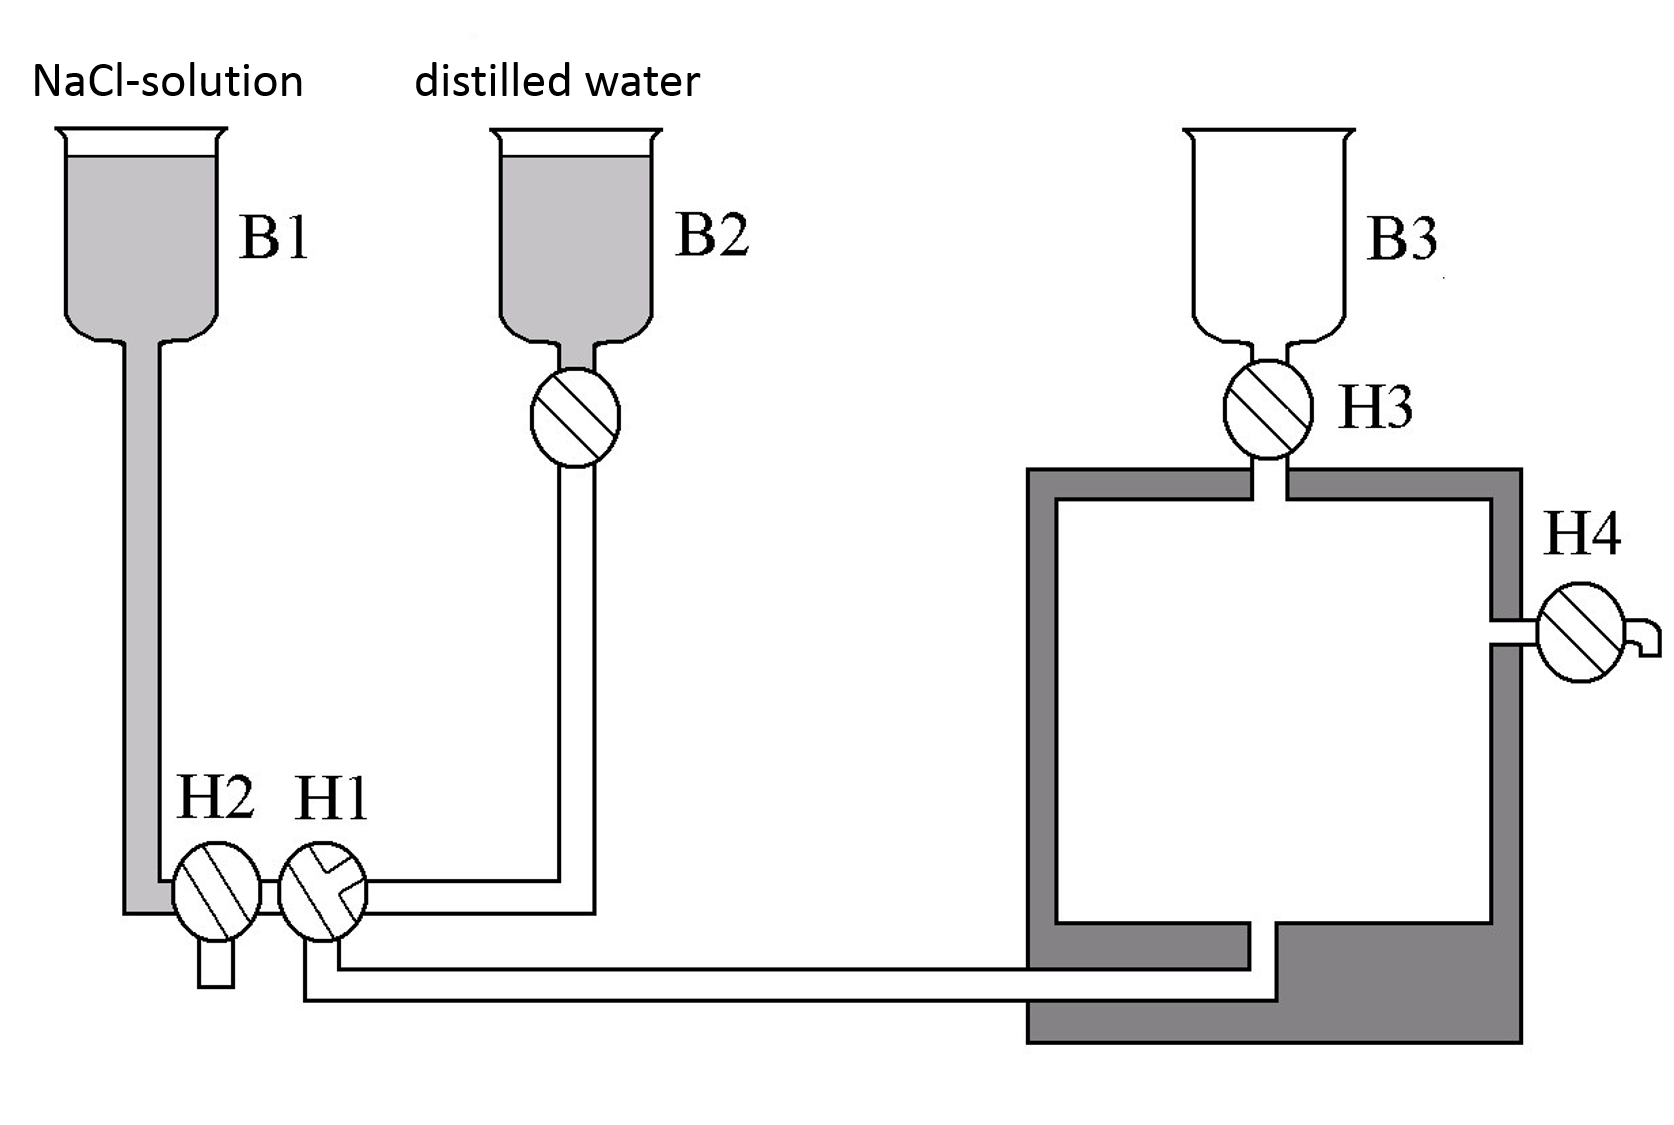
\includegraphics[width=8cm]{GP2-DI-kurz-aufbau_en}} 
\fi 
\captionof{figure}{Diffusion cuvette \label{abb4}}
\vspace{0.05\linewidth}
\end{minipage}

For generation of the interface, following steps are necessary:
	
\begin{itemize}
 \item filling up the reservoir B1 with \ce{NaCl}-solution and B2 with distilled water.
 \item filling up the cuvette (diffusion reservoir) with distilled water from B2 to B3.\\
 \textbf{Attention:} You have to fill up very slowly for avoiding air bubbles in pipe and cuvette. Please consider the setting of the two-way valve H1.
 \item filling in of \ce{NaCl}-solution from B1 under the distilled water, till the interface is over valve H4. \\
 \textbf{Attention:} You have to fill up very slowly to avoid mixing in the residual larger parts of the cuvette.
 \item generation of a sharp interface by using valve for droplet outlet H4.\\
 \textbf{Attention:} As required you have to flow in water from B3 or \ce{NaCl}-solution from B1. 
\end{itemize}


\frage{How is the dependence of the diffusion constant from temperature?}
\frage{ What is the interpretation of the terminology \textit{diffusion velocity} and how is the relation to the diffusion coefficient?}
\frage{Which graphical layout have to be chosen for $Y_{max}=f(t)$ to evaluate the slope in eq. (\ref{diffkoeff})?}
 
\end{document}

